\documentclass[serif,8pt]{beamer}
\usetheme{default} % You can change the theme here
\usecolortheme{metropolis} % You can change the color theme here

% Packages for additional functionality
\usepackage{graphicx} % For including images
\usepackage{amsmath} % For mathematical symbols and equations
\usepackage{multirow}
\usepackage{subfig}

% /home/bogfootlj/.local/share/fonts/NerdFonts
% Setting up fonts

\graphicspath{{./Images/}} % Where to take images from
\setbeamertemplate{section in toc}[sections numbered]
\setbeamertemplate{subsection in toc}[subsections numbered]

% Define the style for the footer with page numbers
\setbeamercolor{footline}{fg=black}
% \addtobeamertemplate{navigation symbols}{}{%
%     \usebeamerfont{footline}%
%     \usebeamercolor[fg]{footline}%
%     \hspace{1em}%
%     \insertframenumber/\inserttotalframenumber
% }

% Define a command to exclude the page counter from the first two slides
\newcommand{\noPageNumber}{%
    \setbeamertemplate{footline}{}%
}

% Define a command to reset the page counter and start numbering from the third slide
\newcommand{\resetPageNumber}{%
    \setbeamertemplate{footline}{%
        \begin{beamercolorbox}[wd=\paperwidth,ht=0.5ex,dp=1ex]{foot}%
            \hspace*{1em}\hfill \insertframenumber/\inserttotalframenumber\hspace*{1em}%
        \end{beamercolorbox}%
    }%
    \addtocounter{framenumber}{-2}%
}

% Set up the footer for the rest of the presentation
\setbeamertemplate{footline}{%
    \begin{beamercolorbox}[wd=\paperwidth,ht=0.5ex,dp=1ex]{foot}%
        \hspace*{1em}\hfill%
        \insertframenumber/\inserttotalframenumber\hspace*{1em}%
    \end{beamercolorbox}%
}


% Title slide information
\title{Generating and teleporting entanglement for quantum networks}
\author{Adrian Udovičić\\
Supervisor:\ Assoc.\ prof.\ dr. Rainer Kaltenbaek}
\institute{University of Ljubljana, Faculty of Mathematics and Physics}
\date{23.05.2024, Ljubljana, Slovenia}
\logo{\includegraphics[height=1cm]{CombinedLogo.png}}

\begin{document}
% Local background must be enclosed by curly braces for grouping.
{\usebackgroundtemplate{\includegraphics[width=\paperwidth,height=\paperheight]{SagnacWithSomeAddedColoursV1.png}}
{\setbeamertemplate{footline}{}

\begin{frame}
	\titlepage
\end{frame}

% \placelogofalse
\usebackgroundtemplate{}
\begin{frame}{Contents}
  \tableofcontents % Include a table of contents slide
\end{frame}

% Example content slides
\resetPageNumber
\section*{Introduction}
\begin{frame}{Introduction}
\end{frame}

\section{Motivation}
\begin{frame}{Motivation}
  \begin{itemize}
	% \item SiQUID
    \item Bright source of entanglement
	\item Training in quantum technologies in Slovenia
	\item Quantum Network for Slovenia
    \item Testbed for industrialized version
	% \item Beyond Semiconductor
	% 	\begin{itemize}
	% 		\item Might also be able to connect multiple nodes with the same source
	% 	\end{itemize}
  \end{itemize}
\end{frame}

\section{Theory}
\begin{frame}{Theory}
	\begin{enumerate}
	\item SPDC
	\item Entanglement swapping
	\end{enumerate}
\end{frame}

\subsection{SPDC}
\begin{frame}{Theory}
	\framesubtitle{SPDC}
		\begin{itemize}
			\item Spontaneous Parametric Downconversion
				\pause
		\end{itemize}

		\begin{figure}
			\begin{center}
				\includegraphics[width=4cm]{SPDC.png}
			\end{center}
			\caption{Illustration of SPDC}\label{fig:SPDC}
		\end{figure}
		\begin{itemize}
			\pause
			\item Non-degenerate
			% \item State of the art
			% \item Different designs
		\end{itemize}
		
\end{frame}

\begin{frame}[t]
	\frametitle{Theory}
	\framesubtitle{State of the Art}
\begin{table}
    \caption{Comparison of different sources}\label{SotA}
    \centering
    \begin{tabular}{|l|l|l|l|l|l|}
        \hline
        Who & \cite{1}  & \cite{2}  & \cite{3}  & \cite{4}  & \cite{5} \\
        \hline
        Type & 0 & II  & II & II & 0  \\
        \hline
		\multirow{2}{*}{\shortstack{Pairs\\(s mW nm)}} & \multirow{2}{*}{2.5 $10^6$} & \multirow{2}{*}{87.5 $10^3$} & \multirow{2}{*}{273 $10^3$} & \multirow{2}{*}{5 $10^3$} & \multirow{2}{*}{278 $10^3$}  \\
		& & & & & \\ % Empty line for spacing
        \hline
        Bandwidth/nm & 106 & 0.3  & 0.3 & 1 & 2.3  \\
        \hline
    \end{tabular}
\end{table}
\end{frame}

\begin{frame}[t]
	\frametitle{Theory}
	\framesubtitle{Different Designs}
	\begin{figure}
		\begin{center}
			% \includegraphics[width=0.95\textwidth]{figures/}
		\end{center}
		\caption{}\label{whoisthis?}
	\end{figure}
\end{frame}

\subsubsection{Phase Matching}
\begin{frame}
	\frametitle{SPDC}
	\framesubtitle{Phase Matching, Quasi Phase Matching, Bandwidth}
	\begin{itemize}
		\item Phase Matching, Quasi Phase Matching
	\end{itemize}

	\begin{figure}
		\begin{center}
		  \subfloat[][]{\includegraphics[width=6cm]{SPDCk.png}}\quad
		\end{center}
		\caption{Illustration of Phase Matching and Quasi Phase Matching.}\label{fig:SPDCk}
	\end{figure}
	
	% \begin{equation}
	% f(\text{T},\text{T0})\text{=}(T-\text{T0}) (T+\text{T0}+546.3)
	% 	\label{eq:Temperature_Dependance}
	% \end{equation}
	% \begin{equation}
	% 	\text{nS}(\text{a},\text{b},\text{T},\lambda)\text{=}\sqrt{ a_1+\text{f}\cdot b_1\frac{a_2+\text{f} \cdot b_2}{\lambda ^2-(a_3+\text{f} \cdot b_3)^2}+\frac{a_4+\text{f} \cdot b_4}{\lambda ^2-a_5^2}-a_6\lambda ^2}
	% 	\label{eq:Refractive_Index}
	% \end{equation}
	\begin{itemize}
		\item Bandwidth
		\item Brightness
	\end{itemize}
\end{frame}

\begin{frame}[t]
	\frametitle{Type-II vs Type-0}
	\framesubtitle{Bandwidth}
	
	\begin{figure}[!ht]
	  \centering
	  \caption{Wavelength bandwidth of a) Type-2 crystal with a polling period of 9,12 um\\ Type-0 crystals with polling periods of b) 19,25 um}
	  \subfloat[][]{\includegraphics[width=5cm]{Type2wavelength.png}}\quad
	  \pause
	  \subfloat[][]{\includegraphics[width=5.5cm]{Type0wavelength.png}}
	  \label{fig:CompT0a2}
	\end{figure}
\end{frame}

\begin{frame}
	\frametitle{SPDC}
	\framesubtitle{Type-2 vs Type-0}

	\begin{table}
		\begin{center}
		\caption{Brightness comparison \[Hz/mW/nm\]}
			\begin{tabular}[c|c|c]{|ll|l|}
				\hline
				\multicolumn{1}{|c}{\textbf{FMF}} & & 
				\multicolumn{1}{c|}{\textbf{IJS}} \\
				\hline 
				\multicolumn{1}{|c|}{\textbf{Type-II}} &
				\multicolumn{1}{c|}{\textbf{Type-0}} &
				\multicolumn{1}{c|}{\textbf{Type-II}} \\
				\hline
				7,8 $\times10^6$ & 2,6 $\times 10^7 $ & 0,05 $\times 10^6 $\\
				\hline
			\end{tabular}
		\end{center}
	\end{table}
	% Overestimated for the "bad" detectors - One has to take into account the dead-time maybe so maybe no one is doing this correctly? :P
\end{frame}

\subsubsection{Detectors}
\begin{frame}
	\frametitle{Detectors}
	\framesubtitle{Dependence of detector dead-time and efficiency}
	\Huge Most important
	\large
Dead-time dependency
\end{frame}

\subsubsection{Efficiency}
\begin{frame}
	\frametitle{SPDC}
	\framesubtitle{Expected efficiency}
	Fiorentino Expected efficiency
	Might not be important
\end{frame}

\subsection{Entanglement swapping}
\begin{frame}{Entanglement swapping}
	\begin{itemize}
		\item FMF/IJS
		\item Quantum Repeaters
			\begin{enumerate}
				\item Quantum Memory - wrong wl for now, have to figure out
			\end{enumerate}
	\end{itemize}

\end{frame}

\section{Present state}

%Temperatures in the 100°C-200°C range are used in order to minimize the photorefractive effect that can damage the crystal and causes the output beam to be distorted.
%Since the photorefractive effect is more severe in PPLN when higher energy photons in the visible part of the spectrum are present in the crystal,
%it is especially important to use the crystal only in the recommended temperature range.
%When using a PPLN crystal as an OPO that is pumped with and generates light in the infrared region of the spectrum,
% it may be possible to use temperatures lower than 100°C if necessary without damaging the crystal.

\subsection{Implementations}
\begin{frame}[t]
	\frametitle{Present state}
	\framesubtitle{Building a linear test setup}
		\begin{itemize}
			\item Focusing parameters
					\begin{equation}
							\xi = \frac{L}{k w^2}
						\label{eq:Focusing parameter}
					\end{equation}
			\item Heralding
				% NOTE: % Might be too much info - Have as backup?
		\end{itemize}

\end{frame}

\subsection{Phase Matching Temperature}
\begin{frame}{Present state}
	\framesubtitle{Phase Matching Temperature}
	\begin{figure}[!ht]
	  \centering
	  % TODO: HAVE TO MAKE THIS BIGGER INCREASE TEXT SIZE IN PYTHON FUCKING NOOB
	  \caption{Temperature scans of Type-0 crystals with different polling periods, a) misaligned 19,25 $\mu$m, b) 19,25 $\mu$m, c) 19,45 $\mu$m, d) 19,65 $\mu$m}
	  \subfloat[][]{\includegraphics[width=2.9cm]{Not_Aligned_Scan.png}}\quad
	  \pause
	  \subfloat[][]{\includegraphics[width=2.9cm]{PMT_Grating_4.png}}\\
	  \subfloat[][]{\includegraphics[width=2.9cm]{PMT_Grating_5.png}}\quad
	  \subfloat[][]{\includegraphics[width=2.9cm]{PMT_Grating_6.png}}\\
	  \label{fig:sub2}
	\end{figure}
\end{frame}

{\usebackgroundtemplate{\includegraphics[width=\paperwidth,height=\paperheight]{SagnacWithSomeAddedColoursV1.png}}
\begin{frame}[t]
	\frametitle{Present state}
	\framesubtitle{Building a Sagnac Interferometer}

	\begin{figure}[!ht]
	  \centering
	  % \subfloat[][]{\includegraphics[width=5cm]{SagnacWithSomeAddedColoursV1.png}}\quad
	  \pause
	  \subfloat[][]{\includegraphics[width=5cm]{PMT_Grating_5.png}}\\
	  \caption{\textcolor{white}{Photograph of the current state of the Sagnac Interferometer.}}
	\end{figure}
\end{frame}

\usebackgroundtemplate{}
\section{Outlook}
\begin{frame}{Outlook}
	\begin{itemize}
		\item SiQUID
		\item Entanglement swapping between FMF and IJS
		\item Building quantum internet
		\item Free space link to reactor
	\end{itemize}
\end{frame}

\begin{frame}{Conclusion}
	\begin{center}
		\Large
		Testing, calculating various properties of the system, limitations, 
	\end{center}
\end{frame}

\begin{frame}{\ }
	\begin{center}
	\Huge
	Thank you
	\end{center}
\end{frame}
\begin{frame}[t]
	\frametitle{References}
\bibliographystyle{IEEEtran}
\bibliography{reference}
	
\end{frame}
\end{document}
